\chapter{Variabili Aleatorie Assolutamente Continue}

Dopo aver analizzato il caso discreto, passiamo ora a studiare una diversa e fondamentale categoria di variabili aleatorie: quelle \emph{assolutamente continue}.  
A differenza delle variabili discrete, la loro probabilità non è concentrata su singoli punti, bensì si distribuisce in modo continuo su un insieme di valori reali.  
In questo contesto, la probabilità che la variabile assuma un valore esatto è nulla, mentre assume significato la probabilità che essa cada all’interno di un intervallo.

\medskip
\noindent Questa rappresentazione permette di esprimere tutte le proprietà probabilistiche di $X$ in termini analitici, utilizzando strumenti del calcolo integrale.\\
\\
Nel seguito introdurremo le principali caratteristiche delle variabili assolutamente continue, analizzando la funzione di densità, la funzione di ripartizione e le loro relazioni, per poi studiare alcuni esempi classici.\\
\\
Prima di dare la definizione di variabile aleatoria continua, dobbiamo definire cosa sia una Probabilità assolutamente continua.

\begin{definizione}
\label{def:9.1}
    Un Probabilità su $\mathcal{B}(\mathbb{R})$ si dice Assolutamente Continua se
    \[\exists\;f:\mathbb{R}\to [0, +\infty]\]
    boreliana, definita \textit{densità continua di }$\mathbb{P}$, tale che la funzione di ripartizione $F$ di $\mathbb{P}$ si scrive come segue:
    \[F(x) = \mathbb{P}((-\infty, x]) = \int_{-\infty}^x f(t)\;dt\quad\left(=\int_{(-\infty, x]}f\;dm\right)\]
\end{definizione}

\noindent Si noti che se $f$ è una densità continua, allora vale che:\[\boxed{\int_\mathbb{R}f(t)\;dt = 1}\]
Difatti:
\[\int_\mathbb{R}f\;dm = \int_{-\infty}^{+\infty}f(t)\;dt = \lim_{n\to+\infty}\underbrace{\int_{-\infty}^n f(t)\;dt}_{F(n)} = \lim_{n\to+\infty}F(n) = 1\]

\begin{teorema}[Caratterizzazione di una Densità Continua]
Valgono i seguenti:
\begin{enumerate}
    \item $f:\mathbb{R}\to\mathbb{R}$ è una densità continua di una probabilità $\mathbb{P}$ assolutamente continua \underline{se e solo se}:
    \begin{enumerate}
        \item $f$ è Boreliana
        \item $f\geq0$
        \item $\int_\mathbb{R}f(x)\;dx = 1$
    \end{enumerate}
    \item Se vale (1.), allora:
    \[\mathbb{P}(A) = \int_Af\;dm = \int_\mathbb{R} f(t)\cdot \mathbb{I}_A(t)\;dm\quad \forall A\in \mathcal{B}(\mathbb{R})\]
    \item $\mathbb{P}$ su $\mathcal{B}(\mathbb{R})$ assolutamente continua è caratterizzata dalla sua densità, ossia:
    \[f_1=f_2\;\text{ quasi certamente}\quad \iff \quad \mathbb{P}_1 = \mathbb{P}_2\]
\end{enumerate}
\end{teorema}

\begin{proposizione}
    Se la funzione di ripartizione $F\in C^0\cap C^1$ a tratti, allora $\exists\,f$ densità continua tale che
    \[f = \begin{cases}
        f(t) = F'(t), \quad & \text{se } \exists \;F'\\
        f(t) = 0 & \text{altrove}
    \end{cases}\]
    e quindi $\mathbb{P}$ associata ad $F$ è assolutamente continua.
\end{proposizione}

\begin{esempio}
    Facciamo due esempi:\\
    \(\bigstar\) Sia $F(t) = (11 - e^{-\lambda t})\mathbb{I}_{(0, +\infty)}$  con associata la sua probabilità $\mathbb{P}$. \\
    Allora siccome $F$ è ovunque derivabile tranne che nello zero, si ha che $\mathbb{P}$ è  assolutamente continua e la sua densità vale:
    \[f(t) = \begin{cases}
        \lambda e^{-\lambda t}, \quad &\text{se } t>0\\
        0,  \quad &\text{se } t \leq 0
    \end{cases}\]

    \(\bigstar\) Sia $F(t) = \frac{t-a}{b-a}\mathbb{I}_{[a, b]}(t) + \mathbb{I}_{(b, +\infty)}$. 

    \begin{figure}[H]
\centering
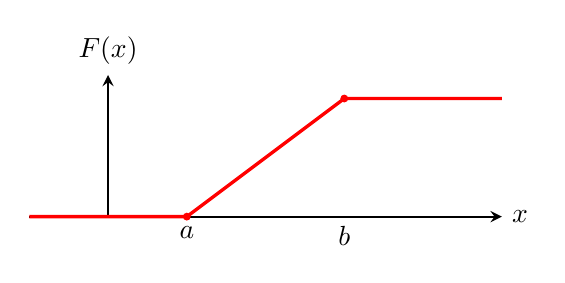
\begin{tikzpicture}[x=1cm,y=1.5cm,>=stealth]

% --- Assi ---
\draw[->, thick] (-1,0) -- (5,0) node[right] {$x$};
\draw[->, thick] (0,0) -- (0,1.2) node[above] {$F(x)$};

% --- Funzione a tratti ---
\draw[very thick, red]
  (-1,0) -- (1,0)
  -- (3,1)
  -- (5,1);

% --- Punti a e b ---
\filldraw[red] (1,0) circle (1.2pt);
\filldraw[red] (3,1) circle (1.2pt);

% --- Etichette ---
\node[below] at (1,0) {$a$};
\node[below] at (3,0) {$b$};

% --- Griglia opzionale ---
% \draw[step=0.5cm, gray!30, very thin] (-1.2,-0.1) grid (5.2,1.2);

\end{tikzpicture}
\end{figure}


    Si vede disegnando la funzione che $F\in C^1$ a tratti ed è continua, allora $\mathbb{P}$ è  assolutamente continua e vale che:
    \[f(t) = \begin{cases}
        \frac{1}{b-a}, \quad &\text{se }t\in[a, b]\\
        0, \quad &\text{altirmenti }
    \end{cases} \;=\frac{1}{b-a} \mathbb{I}_{[a, b]}(t)\]
\end{esempio}

Si noti che nell'ultimo esempio si poteva tranquillamente prendere $\tilde{f}(t) = \frac{1}{b-a} \mathbb{I}_{(a, b)}(t)$, tanto a noi interessa la classe di equivalenza del rappresentante (che è per esempio $f(t))$.\\
\\
Inoltre, se $\mathbb{P}$ è assolutamente continua, allora $F(t) = \int_{-\infty}^tf(x)\;dx$ è una funzione continua.

\begin{definizione}
    $X:\Omega\to\mathbb{R}$ è Assolutamente Continua se $P^X$ è una misura di probabilità Assolutamente Continua, e definiamo $f_X$ la sua densità.
\end{definizione}

\noindent Si osservi che data $a\leq X\leq b$ quasi certamente, con $a, b\in\mathbb{R}$, allora:
\[\mathbb{P}(X\in[a, b]) = 1\quad \iff \quad f_X(t)=0\;\text{ quasi certamente }\;\forall t \in [a, b]^c\]

\begin{teorema}[Regola del Valore Atteso Continuo]
    Sia $X:\Omega\to\mathbb{R}$ una variabile aleatoria assolutamente continua con legge $P^X$ e densità $f_X$.\\
    Sia $h:\mathbb{R}\to\mathbb{R}$ boreliana, allora:
    \begin{enumerate}
        \item La composizione $h(X)$ è tale che
        \begin{align*}
        h(X)\in L^1(\Omega, \mathcal{A}, \mathbb{P}) \quad & \iff \quad h\in L^1(\mathbb{R}, \mathcal{B}, P^X)\\
        & \iff \quad h\cdot f_X\in L^1(\mathbb{R}, \mathcal{B}, m)\\
        & \iff \quad \int_\mathbb{R} \left|h(x)\right|\cdot f(x)\;dx <+\infty
\end{align*}
        \item Se $h\in L^1(P^X),\;$ oppure se $h:\mathbb{R}\to[0, +\infty]$, allora:
        \[\boxed{E[h(X)] = \int_\Omega h(X)\;d\mathbb{P} = \int_\mathbb{R} h\;dP^X \overset{\footnote{In questa uguaglianza (e nella seconda implicazione del punto 1.) si usa il fatto che se $X$ è assolutamente continua, allora $dP^X = f_X\cdot dm$. Per chi voglia approfondire, questo deriva dal Teorema di Radon–Nikodým.}}{=} \int_\mathbb{R}h(x)\,f_X(x)\;dx}\]
    \end{enumerate}
\end{teorema}
\noindent Possiamo osservare (come abbiamo fatto nel caso discreto) due fatti importanti:
\begin{enumerate}
    \item $X\in L^1(\Omega, \mathcal{A}, \mathbb{P}) \quad  \iff \quad \int_\mathbb{R}|t|\,f_X(t)\;dt<+\infty\qquad \Rightarrow\qquad \boxed{E[X] = \int_\mathbb{R}tf_X(t)\;dt}$.
    
    \item $X\in L^2(\Omega, \mathcal{A}, \mathbb{P}) \quad  \iff \quad \int_\mathbb{R}t^2f_X(t)\;dt<+\infty \qquad \Rightarrow\qquad \boxed{Var(X) = \int_\mathbb{R}(t-\mu)^2f_X(t)\;dt}$
\end{enumerate}

\begin{teorema}
    Sia $\mathbb{P}$ su $\mathcal{B}$ assolutamente continua con densità $f$, e sia $A\in\mathcal{B}$ tale che $m(A) = 0$.
    \[\Rightarrow\quad \mathbb{P}(A) = 0\]
    \begin{dimostrazione}
        \[\mathbb{P}(A) = \int_A f\;dm = \int_\mathbb{R} f \mathbb{I}_A\; dm\]
        Dove per ipotesi si ha che:
        \[m(A) = \int_\mathbb{R}\mathbb{I}_A\;dm = 0\quad \Rightarrow\quad \mathbb{I}_A\in[0]\]
        ovvero che $\mathbb{I}_A = 0\;$ quasi ovunque.

        \medskip
        \noindent Di conseguenza:
        \[\int_\mathbb{R}f\mathbb{I}_A\;dm = 0= \mathbb{P}(A)\]
    \end{dimostrazione}
\end{teorema}
\begin{esempio}
    Sia $X\sim\mathcal{U}([a, b])$, ossia che
    \[f_X(t) = \frac{1}{b-a}\cdot \mathbb{I}_{[a, b]}(t)\]
    Allora $X\in L^1\;$ e $\;a\leq E[X]\leq b$, infatti:
    \[E[X] = \int_a^b\frac{t}{b-a}\;dt = \frac{b+a}{2}\in[a, b]\]
\end{esempio}
\begin{esempio}
    Sia $X\sim \mathcal{E}(\lambda)$, ossia che
    \[f_X(t) = \lambda e^{-\lambda t} \;\mathbb{I}_{\{t\geq0\}}\]
    Ci chiediamo, $X\overset{?}{\in }L^1$?
    Ricordandoci che:
    \[\Gamma(\alpha) = \int_0^{+\infty} x^{\alpha -1} e^{-x}\;dx;\qquad \text{Se }\;\alpha = n+1\quad \Rightarrow\quad \Gamma(n+1) = n!\quad \text{con}\;n\geq0\]
    Allora possiamo calcolare il valore atteso: 
    \[E[X] = \int_0^{+\infty} t\lambda e^{-\lambda t}\;dt \overset{t\lambda = x}{=} \frac{1}{\lambda} \int_0^{+\infty} x e^{-x}\;dx = \frac{\Gamma(2)}{\lambda}=\frac{1}{\lambda}<+\infty \]
    Abbiamo appena dimostrato che se $X\sim\mathcal{E}(\lambda),\;\lambda>0$, allora $X\in L^1$.
\end{esempio}
\begin{esempio}
    Si prenda $X:\Omega \to \mathbb{R}$ distribuita con una densità di Cauchy:
    \[f_X(t) = \frac{1}{\pi}\frac{1}{(1+t^2)}\]
    Ci chiediamo di nuovo, $X\overset{?}{\in }L^1$?
    
    \[E[|X|] \;=\; \int_{\mathbb{R}} |t|\, f_X(t)\,dt
= \frac{1}{\pi}\int_{\mathbb{R}} \frac{|t|}{1+t^2}\,dt
= \frac{2}{\pi}\int_{0}^{\infty} \frac{t}{1+t^2}\,dt = +\infty\]
Ne segue quindi che $X\notin L^1$. Addirittura sia ha che la densità di Cauchy non possiede nessun momento assoluto $p$--esimo finito, difatti:
\[E[|X|^p] <+\infty \quad \iff \quad p<1\]
dato che all'infinito si ha che
\[\frac{|t|^p}{1+t^2}\sim\frac{1}{t^{2-p}}\]
    
\end{esempio}



\section{Riassunto Utile e Considerazioni Pratiche}
Sia  $f_X:\mathbb{R}\to [0, +\infty]$ tale che sia una densità continua. Ci chiediamo: \textit{esiste sempre finito il valore atteso $E[X]$?}.\\
Abbiamo tre casi da vedere:
\begin{itemize}
    \item[\(\bigstar\)] $f_X(t) = 0$ su $[a, b]^c \quad  \iff \quad \mathbb{P}(X\in[a, b]) = 1 = P^X([a, b]) \quad  \iff \quad a\leq X\leq b$\\
    \\
    $\Rightarrow \qquad X\in L^1\quad \text{e}\quad a\leq E[X] \leq b$
    
    \medskip
    \noindent Il solo fatto che $f_X$ si annulli sul complementare di un intervallo chiuso, mi implica che esista il valore atteso.
    \item[\(\bigstar\)] $f_X(t) = 0$ su $(-\infty, 0) = [0, +\infty)^c \quad  \iff \quad \mathbb{P}(X\in[0, +\infty)) = 1$\\
    \\
    $\Rightarrow \qquad \exists$ il valore atteso, ma si hanno due possibilità :\quad $\begin{cases}
        +\infty\\
        c\in\mathbb{R}^+\qquad \Rightarrow X\in L^1(\mathbb{P})
    \end{cases}$
    \item[\(\bigstar\)] $f_X(t) \neq0\;\;\forall t\in\mathbb{R}$\\
    In questo caso bisogna prima verificare che $E[X]$ esista\\
    \[\text{Se }\quad E[|X|] = \int_\mathbb{R}|t|f_X(t)\;dt<+\infty \qquad \Rightarrow\quad X\in L^1\]
    e nel caso calcolarlo come
    \[E[X] = \int_\mathbb{R}tf_X(t)\;dt\]
\end{itemize}

\bigskip
\noindent Riassumiamo ora le relazioni tra le condizioni per decretare se una V.A. è continua.\\
\\
Dato uno spazio di probabilità $(\Omega, \mathcal{A}, \mathbb{P})$ e una variabile aleatoria $X : \Omega \to \mathbb{R}$.\\
Allora $X$ è Assolutamente Continua:
\begin{align*}
    & \iff P^X \text{ ammette densità } f, \quad P^X(B) = \int_B f(x)\,dx \quad \forall B \in \mathcal{B}\\
    & \iff F_X(t) = \int_{-\infty}^{t} f(x)\,dx \quad \forall t \in \mathbb{R}\\
    & \;\;\Longrightarrow F_X \in C^0, \quad \text{ovvero } P^X(\{x\}) = 
    \mathbb{P}(X = x) = F_X(x) - F_X(x_-) = 0 \\
    & \;\Longleftarrow F_X \in C^0 \cap C^1 \text{ a tratti}
\end{align*}

In quest’ultimo caso:
\[
f(x) =
\begin{cases}
F_X'(x), & \text{dove } F_X \text{ è derivabile} \\
\text{valore arbitrario}, & \text{altrimenti.}
\end{cases}
\]



